\section{Proof Automation}\label{automated-sec}

In this project we used proof automation in two ways: automated theorem provers (ATPs) and \emph{Lean} tactics.
ATPs are generally stand-alone tools that implement a (semi-)decision procedure for a given formal language or related set of languages.
For example, \emph{Vampire}~\cite{DBLP:conf/cav/KovacsV13} is an ATP focused primarily on first-order logic using superposition, which we used extensively in this project.  We also made extensive use of \emph{Prover9} and \emph{Mace}~\cite{prover9-mace4}.

ATPs are complex software that can contain bugs.
Instead of trusting ATP output, we used proof certificates, which many ATPs can produce, to reconstruct proofs in \emph{Lean}.
The details of proof reconstruction depend on the form of the proof certificate produced by the ATP.
We expand on this in \Cref{sec:proof-reconstruction}.

Tactics in \emph{Lean}, on the other hand, are meta-programs~\cite{DBLP:journals/pacmpl/EbnerURAM17} that build proofs.
In other words, they essentially take \emph{Lean} code as input and produce \emph{Lean} code as output.
In this manner, they look like another keyword in the language, and are tightly integrated by producing proofs directly.
Under the hood, their implementation can be arbitrarily complex, from syntactic sugar to full decision procedures.
The \texttt{duper} tactic~\cite{DBLP:conf/itp/CluneQBA24}, for example, implements a superposition calculus, similar to \emph{Vampire}'s, but for dependent types --- \emph{Lean}'s underlying logical foundation.

In the rest of this section we describe the different proof automation techniques used in this project.
We first discuss the different proof methods used: primarily superposition and equational reasoning, we then discuss the integration in \emph{Lean}, and finally we report some basic empirical results from this project.

\subsection{Proof Techniques}

The main two families of ATPs and tactics we used are based on superposition/saturation and equational reasoning.
In this context we also include SMT solvers, which combine specific decision procedures for theories, like congruence closure for equational reasoning, with satisfiability (SAT) solving \cite{deMoura-Bjorner-2009}.
Finally, we also used \texttt{aesop}~\cite{DBLP:conf/cpp/LimpergF23}, which implements a version of tableau search.
This was used mainly to help specific constructions in refutations, and is not specific to proving or disproving magma implications in this sense.
We describe our use of \texttt{aesop} in \Cref{sec:proof-reconstruction} below.

\textbf{Saturation.}
Most of the ATPs used extensively in this project rely primarily on saturation procedures in the superposition calculus.
For example, this is the case for \emph{Vampire}~\cite{DBLP:conf/cav/KovacsV13}.\footnote{See also~\cite{DBLP:journals/cacm/BentkampBNTVW23} for a gentler exposition.}
The core idea of these provers is that they take a set of assumptions and a conjecture, expressed in --- say --- first-order logic.
The conjecture is negated and added to the set of assumptions, which are all put into a normal form.
The ATP then tries to refute the negation by applying rules of an underlying calculus, until a proof of false (a contradiction) is derived.
In this case, the conjecture was (classically) true, and the ATP has found a proof by contradiction, often called a ``refutation'' or ``saturation'' proof.

The underlying calculi vary from system to system, but they often have a variant of a resolution clause of the form:
\[\infer{C \lor D}{C \lor L \quad D \lor \neg L} \]
This can be read as $C \lor L$ with $D \lor \neg L$ implies $C \lor D$, where $C, D, L$ are formulas in e.g. first-order logic.
Superposition calculi have a variant of this rule that deals with equality directly, and thus are more efficient at reasoning about equality.

In this project we used \emph{Vampire}~\cite{DBLP:conf/cav/KovacsV13}, \emph{Duper}~\cite{DBLP:conf/itp/CluneQBA24} and \emph{Prover9} and \emph{Mace4}~\cite{prover9-mace4} which are all based on variants of saturation for proving.

\textbf{Equational Reasoning.} As already discussed in \Cref{canon-sec}, equational reasoning is a type of reasoning that is based\footnote{More precisely, one can formalize this reasoning using Birkhoff's five rules of inference (reflexive, symmetric, transitive, replacement, and substitution); see, e.g., \cite{burris}.} on equational logic and rewriting with congruence~\cite{term-rewriting}.
In general, an equational reasoning procedure takes a series of equations and tries to determine whether another equation can be deduced from it.
A core tool in equational reasoning are \emph{e-graphs}, a data structure used to represent congruence classes of terms.
By themselves, e-graphs provide an efficient means of implementing a decision procedure for congruence closure over ground equations (i.e. equations without variables).
Extensions to this procedure, for example by quantifier instantiation via e-matching \cite{DBLP:conf/cade/MouraB07}, also allow for a semi-decision procedure for congruence closure over non-ground equations.

SMT solvers like \emph{Z3}~\cite{DBLP:conf/tacas/MouraB08} use equational reasoning for deciding the theory of equality with uninterpreted functions~\cite{DBLP:series/txtcs/KroeningS16,DBLP:conf/cade/MouraB07}.
On the other hand, equality saturation~\cite{DBLP:journals/pacmpl/WillseyNWFTP21} uses e-graphs by extending congruence closure to a more controlled search, enabling optimization and conditional rewriting.
One of the main advantages of using equational reasoning to reason about implications of magma laws is that we get very explicit proofs: a proof that $l \models l'$ is given by a sequence of rewrites that starts at the left-hand side of $l'$ and arrives at the right-hand side through applications of $l$.

In this project we used \emph{Z3}~\cite{DBLP:conf/tacas/MouraB08}, \emph{Prover9} and \emph{Mace4}~\cite{prover9-mace4}, a custom ATP \emph{MagmaEgg} for magmas based on egg~\cite{DBLP:journals/pacmpl/WillseyNWFTP21}, and the \emph{Lean} \texttt{egg} tactic~\cite{DBLP:journals/pacmpl/KoehlerGBGTS24,rossel2024equality}, which all work with equational logic. We have also reasoned with manual (custom written) heuristics about simple rewrites.

\subsection{Integration of Automation Procedures}
\label{sec:proof-reconstruction}

While ATPs are very useful for solving theorems in this project, they do not integrate with \emph{Lean} out of the box.
ATPs may produce unsound proofs, or worse, derive incorrect results.
Thus, by default, theorems in \emph{Lean} cannot be proven by deferring to the result of an ATP.
Instead, the results of an ATP can be used to reconstruct a proof of the form required by \emph{Lean}.
% There are different approaches to proof reconstruction which we employ in this project.
Thus, in general, integration of ATPs requires two steps.
First, there is the invocation of the ATPs by translating the problem from \emph{Lean} into the languages and logics they use.
And second, there is the reconstruction of the ATPs' results as a (persistent) \emph{Lean} proof.
These two aspects present different challenges, and require different strategies, depending mostly on the kind of proof strategy the ATP uses.

More generally, we have observed that there are multiple ways of integrating decisions procedures within \emph{Lean}, with different levels of integration.

\begin{enumerate}
    \item Using a \emph{Lean} tactic, which calls a decision procedure written in \emph{Lean} (like \texttt{aesop} or \texttt{duper}).
    \item\label{inter} Using a \emph{Lean} tactic, which calls an existing (external) ATP and reconstructs a proof term from the ATP's result (like \texttt{bv\_decide} or \texttt{egg}).
    \item\label{external} Using an external script which calls an existing ATP and generates a source file \texttt{.lean} which captures the result explicitly.
\end{enumerate}

This project primarily used the least integrated approach, Option \ref{external}, as it was fastest to implement and imposed no additional technical requirements on other contributors.
The matter of technical requirements caused problems, for example, when integrating the \texttt{egg} tactic (Option \ref{inter}) as it initially expected certain software on the user's machine.
Such trade-offs between Option \ref{inter} and Option \ref{external} are, however, mutual, as the higher upfront cost of integrating a proof tactic in Option \ref{inter} makes the decision procedure easier to use than with Option \ref{external}.
Additionally, Option \ref{inter} can benefit from \emph{Lean}'s meta-programming capabilities when encoding the problem for use with an ATP, and when reconstructing a \emph{Lean} proof from the result.

\textbf{Proof Reconstruction.}

The relative simplicity of the objects used in this project benefit the implementations of proof reconstruction.
By focusing on the given problem domain, difficult reconstruction issues, like complex dependent types, could be ignored.

For saturation proofs with \emph{Vampire}, we implemented analogs of the \emph{superpose}, \emph{resolve}, and \emph{subsumption} steps in \emph{Lean}.
Proofs can then be reconstructed as sequences of these steps (and additional technicalities) as shown in Figure~\ref{fig:vampire-example}.

\begin{figure}
  \centering
  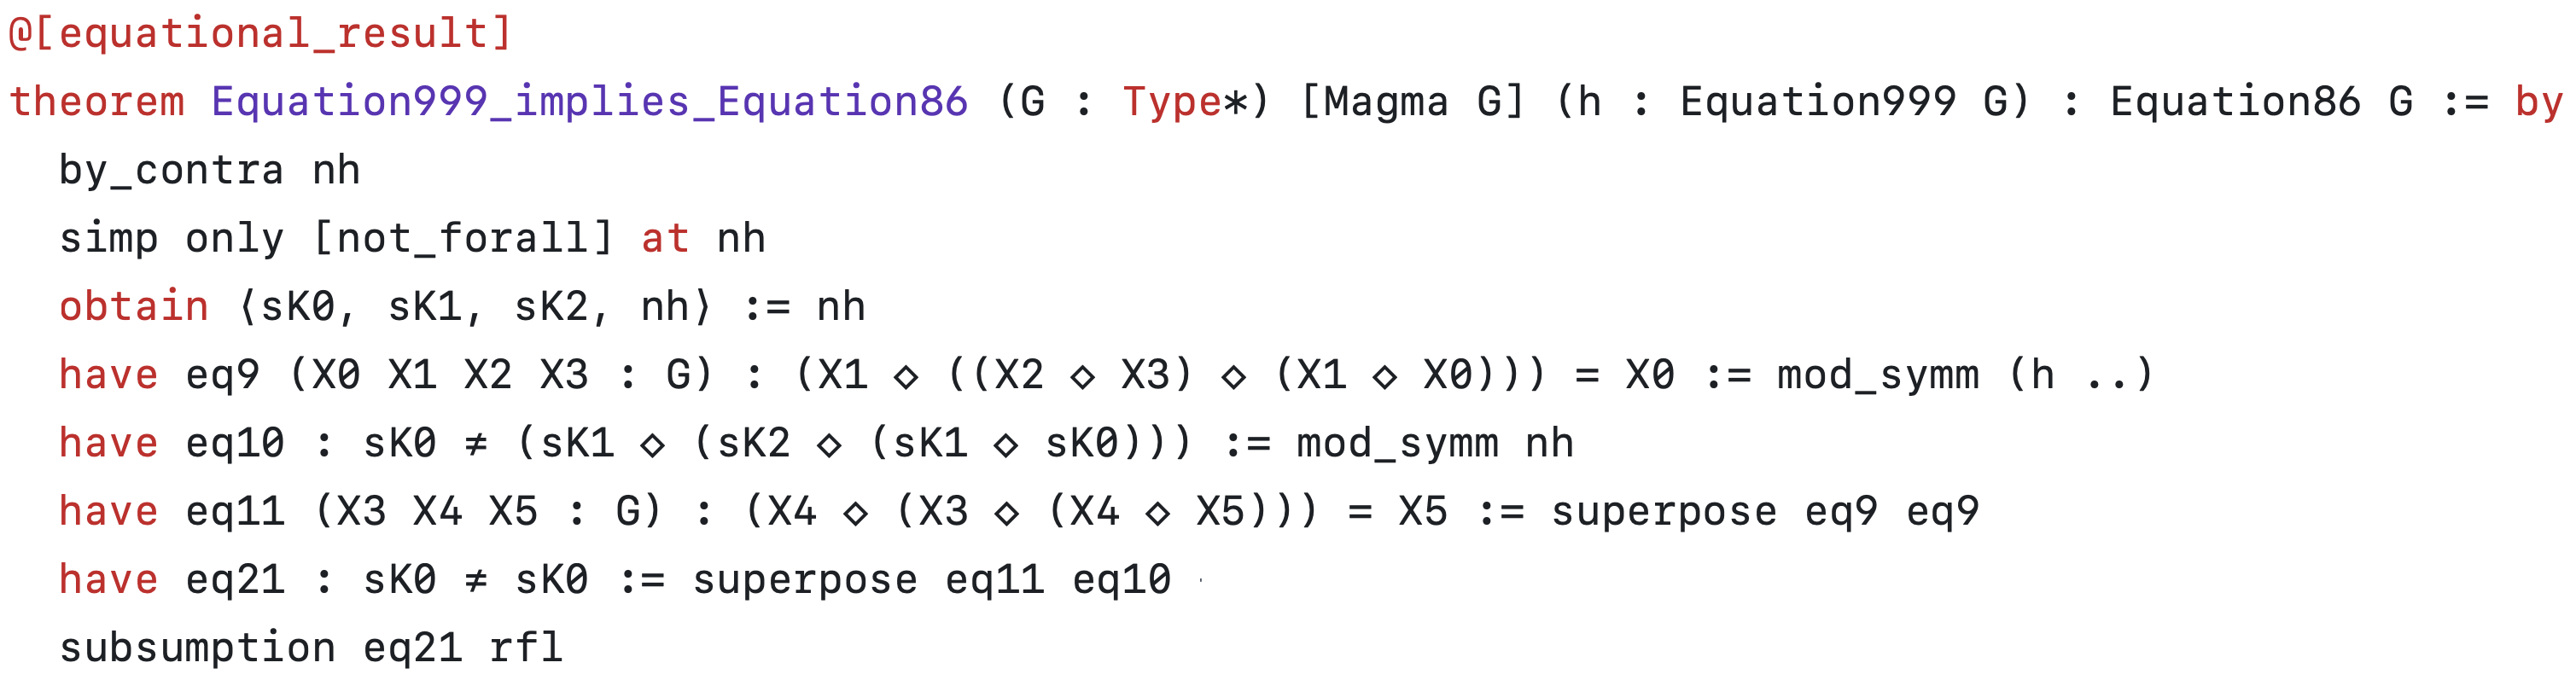
\includegraphics[width=\textwidth]{vampire-example.png}
  \caption{Example of a proof reconstructed from output of \emph{Vampire}. Note how the proof proceeds by contradiction and uses the \texttt{superpose} and \texttt{subsumption} steps implemented in \emph{Lean}.}
  \label{fig:vampire-example}
\end{figure}
% \todo{Use listings or minted for this code block.}

% \todo{Explain how Prover9 and Mace4 were used.}

For equational proofs from external provers, like \emph{MagmaEgg}, we also used a tailored version of reconstruction.
Specifically, the \emph{MagmaEgg} implementation turns \emph{explanations} \cite{nieuwenhuis2005proof} from \emph{egg} into \emph{Lean} proofs by simple applications of the defining properties of equality as shown in Figure~\ref{fig:magma-egg-example}.

\begin{figure}
  \centering
  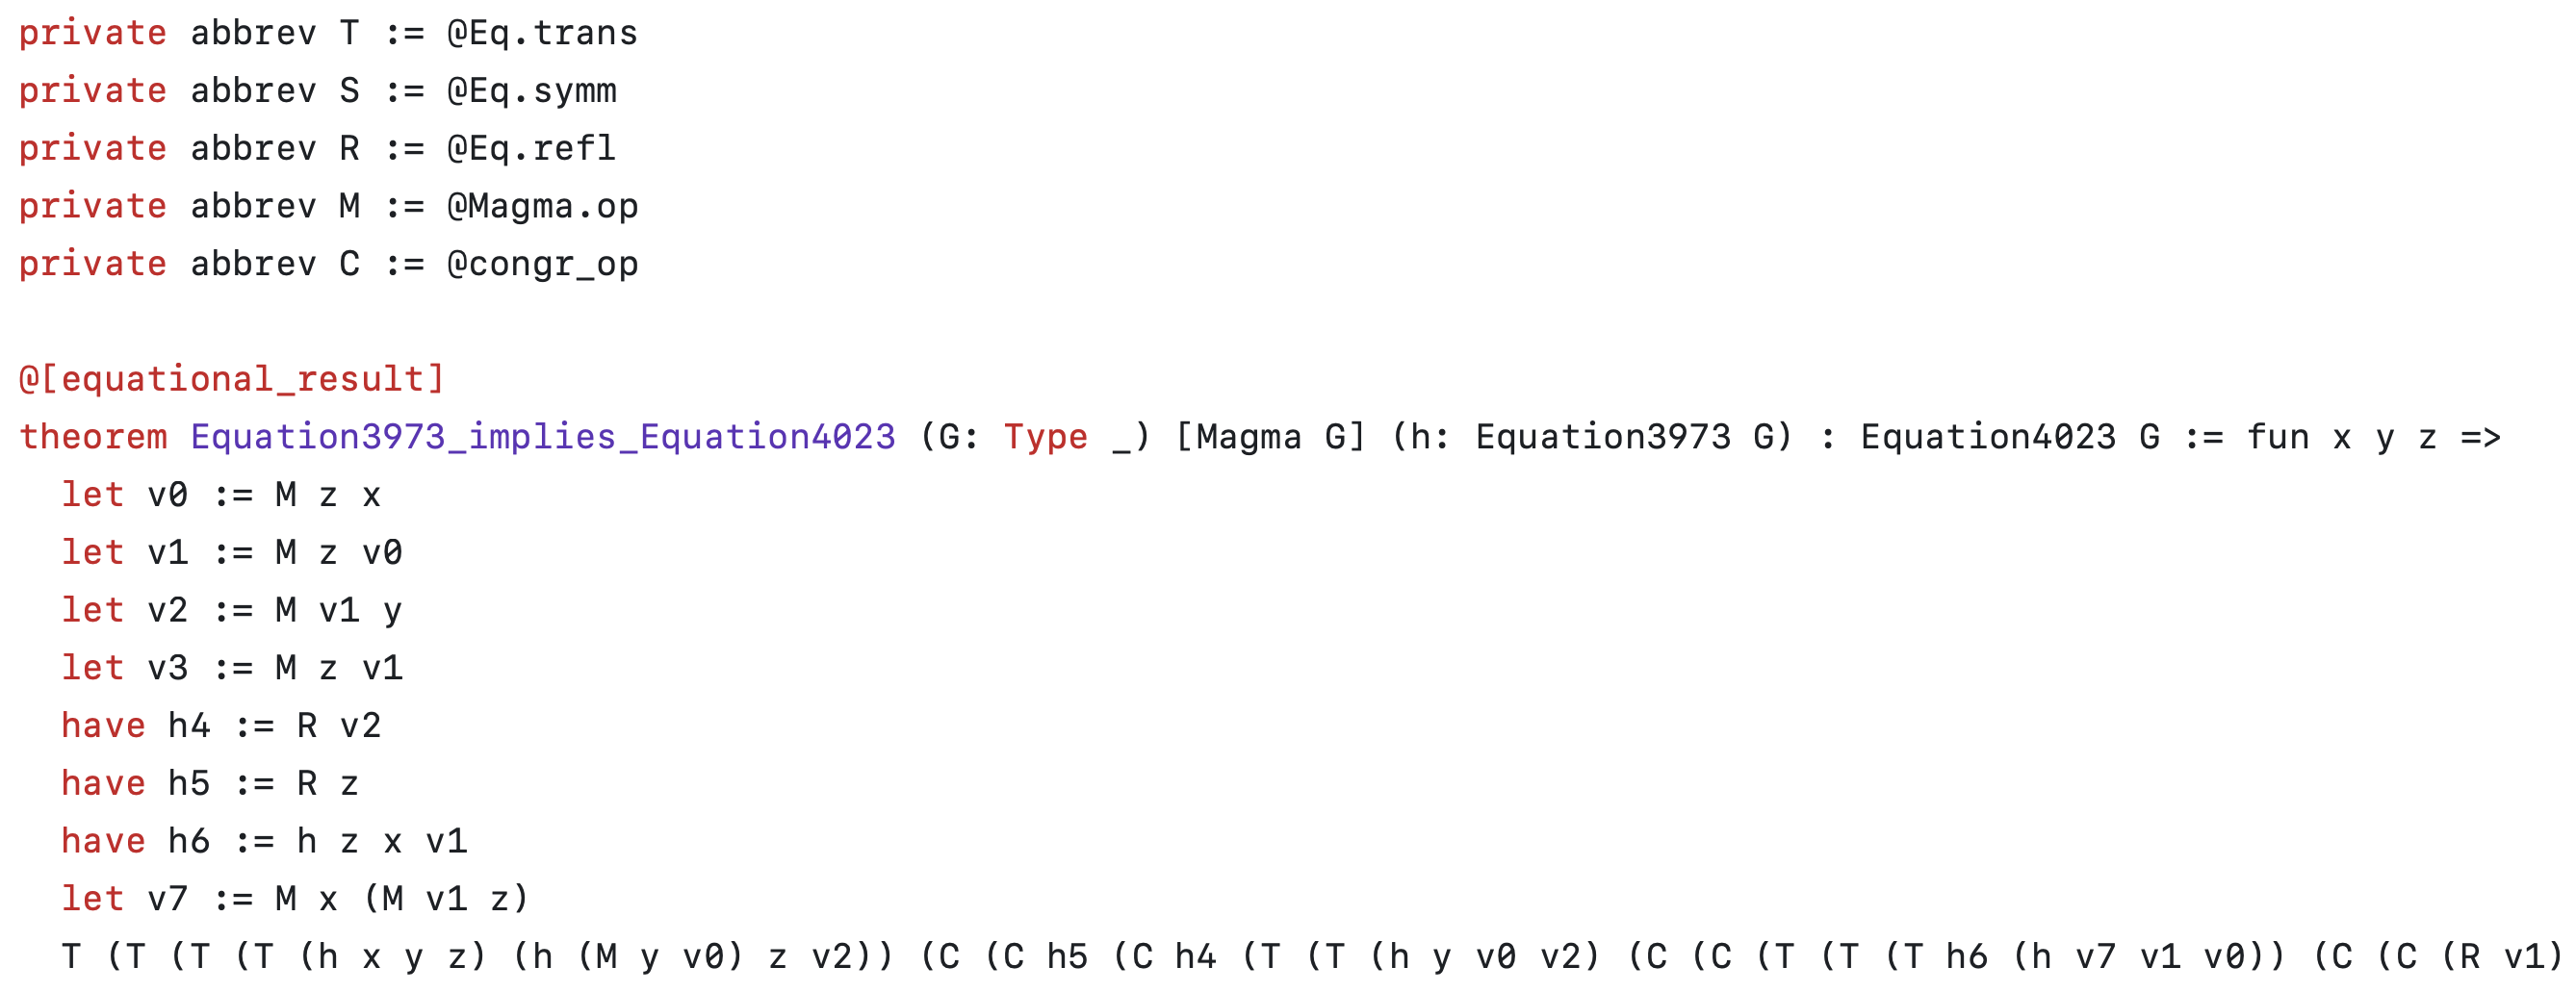
\includegraphics[width=\textwidth]{magma-egg-example.png}
  % SOURCE: https://github.com/teorth/equational_theories/blob/main/equational_theories/Generated/MagmaEgg/small/_005.lean
  \caption{Example of a proof reconstructed by \emph{MagmaEgg}. Note the proof only uses reflexivity, symmetry, transitivity, and congruence of equality.}
  \label{fig:magma-egg-example}
\end{figure}
% \todo{Use listings or minted for this code block.}

In the case of the \texttt{egg} tactic, which also reconstructs proofs from \emph{egg} explanations, the proof could be converted into a more human-readable form by using the \texttt{calcify}\footnote{\url{https://github.com/nomeata/lean-calcify}} tactic, as shown in Figure~\ref{fig:egg-example}

\begin{figure}
  \centering
  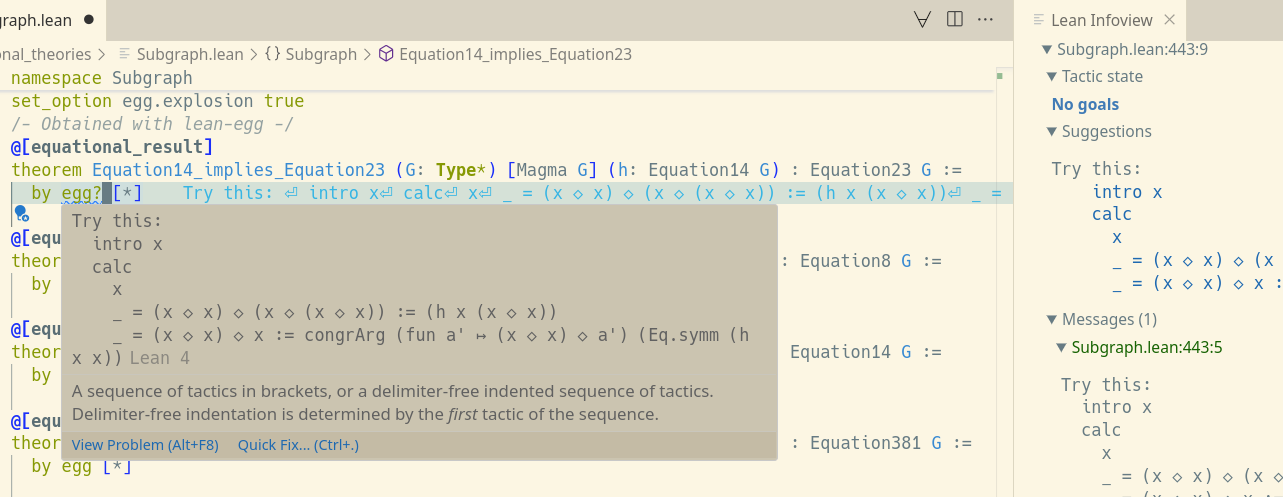
\includegraphics[width=\textwidth]{egg-example.png}
  \caption{Example of the \texttt{egg} tactic reconstructing a proof in human-readable form with the help of \texttt{calcify} (invoked by the special syntax \texttt{egg?}).}
  \label{fig:egg-example}
\end{figure}

\textbf{Semi-Automated Counterexample Guidance.}  Another use of ATPs has been in a semi-automatic fashion, to find counterexamples.
The general strategy was to use ATPs to find counterexamples to implications by building magmas iteratively.
If we want to build a counterexample to $l \models l'$, we want to construct a magma where $l$ holds but $l'$ does not.
In this method, we iteratively strengthen a construction with additional hypotheses, and use the ATP to check whether these hypotheses are not too strong (to imply $l'$) or unsound (to disallow $l$).

% \TODO{this should also be expanded more, at least with references to some of the constructions in other chapters.}

While equational reasoning can also be used in a semi-automatic fashion to prove equations~\cite{DBLP:journals/pacmpl/KoehlerGBGTS24}, the positive implications in the main implication graph of project were all simple enough that we did not need a semi-automatic approach for them.

% \TODO{discuss guided search in the finite implications or the Higman-Neumann work Jose Brox has done.}

% \TODO{maybe add a screenshot here of the workflow of using a seed to find counterexamples with \emph{Prover9} or \emph{Vampire}?}

% \subsection{Empirical Results}

% Finally, we report some empirical results from use of ATPs for this project, in terms of performance.
% This section is not intended to be a careful evaluation and benchmark comparison of the different ATPs; instead, we present our work here as a more informal ``field report'' documenting our experiences.
% In particular, we do not draw firm conclusions about the overall capabilities\footnote{One reason for this is that different ATPs were deployed at different stages of the project.  In particular, the later ATP runs were performed in an environment when a large fraction of the implications had already been settled, and only a small remainder set was tested by our project.  The current set of ATP-generated formalized implications has also been subject to a number of reductions to optimize compilation time, so we would caution against reading too much into the raw number of such formalizations in the codebase.} of the different ATPs.
% Rather, this serves as a use-case documenting the experience of (mostly) novice users.

% \TODO{throw a couple of "benchmarking" tables for the same ATP with different parameters and for different ATPs, talk about some relative gains in time (changing parameters we saw a 500 times speedup on this particular problem), etc. This is knowledge I think we have gained to some extent, and certainly I would have been glad to receive this kind of hints before we started!''.  Then leave it as an interesting open problem to properly develop and measure benchmarks for ATPs based on this project.}

% {\bf Any comparative study of semi-automated methods with fully automated ones? In principle, the semi-automated approach could be more automated using a script or "agent" to call various theorem provers. See \href{https://leanprover.zulipchat.com/#narrow/stream/458659-Equational/topic/A.20magma.20of.20order.20.3C.2013.20-.20for.20Equation2531.3F}{this discussion}}


% {\bf See \href{https://leanprover.zulipchat.com/#narrow/channel/458659-Equational/topic/1516.20-.3E.20255/near/481547543}{this discussion} on the value of using different ATPs and setting run time parameters etc. at different values.}

% {\bf What are the hardest implications to prove?  See \href{https://leanprover.zulipchat.com/#narrow/channel/458659-Equational/topic/What.20are.20the.20hardest.20positive.20implications.20for.20an.20ATP.3F}{this discussion}.}
